\begin{frame}
  \begin{center}
    {\huge A* Sampling
    } \\
    Maddison,Tarlow,Minka
  \end{center}
\end{frame}

%%%%%%%%%%%%%%%%%%%%%%%%%%%%%%%%%%%%%%%%%%%%%%%%%%
%% \begin{frame}{Introduction - Partition Function Woes}
%%   \begin{itemize}[<+->]
%%   \item Gibbs Distribution
%%     \begin{align*}
%%       \Pr(\x;\theta) =\frac{\exp(\theta^T\psi(\x))}{Z(\theta)} \tag{$Z=\sum_{\x} \theta^T\psi(\x)$}
%%     \end{align*}
%%     %% A standard/popular way of probabilistic modeling 
%%   \item Parameter Estimation,
%%     \begin{align*}
%%       - \frac{1}{T}\nabla_\theta \sum_i\log LLH = \E_{\Pr(x;\theta)}\left[\psi(\x)\right] - \frac{1}{T} \sum_i\psi(x_i)
%%     \end{align*}
%%     %% suppose you are doing parameter estimation using MLE.
%%   \item Computing $\E_{\Pr(x;\theta)}[.]$ often intractable.
%%     %% may have to sum over exponential # of states
%%   \item So we resort to approximations.
%%     %% Sampling from posterior is hard
%%     %% MCMC, Contrastive Divergence
%%     %% sampling is inherently tied to Z
%%     %% but computing Z is #P hard in general
%%     %% This paper provides a way to obtain exact samples from a intractable distribution.
%%   \end{itemize}
%% \end{frame}

%%%%%%%%%%%%%%%%%%%%%%%%%%%%%%%%%%%%%%%%%%%%%%%%%%
\begin{frame}[label=framelabel]{Gumbel Distribution}
  %% First lets establish the mathematical machinery 
  \begin{itemize}[<+->]
  \item Distribution of maximas of samples from exponential-like distributions.
    %% We will work with Gumbel with location parameter only.
  \item CDF for $Gumbel(m)$, $\Pr(G\le g) = \exp(-\exp(-g+m))$
    %% Mean is $m+\gamma$, Variance is $\frac{\pi^2}{6}$.
  \end{itemize}
      \begin{figure}
        \centering

        \begin{tikzpicture}[scale=0.8] % plotting with data in columns
          \begin{axis}[
              ymax=0.5,
              xlabel=x,
              ylabel=y,
              legend style={
                at={(0.5,-0.18)},       % 0.5 times xmin,xmax and -0.18 times ymin,ymax, think affine comb.
                anchor=north,
                legend columns=-1       % no columns, only rows
              },
              extra x ticks={0},  % Add an extra tick at position x=1
              extra x tick style={    % Set styles that only apply to the extra tick
                xticklabel pos=right,   % Put the label on the right ( = top) side of the plot
                xticklabels={m}, % Set the label text
                xmajorgrids=true,            % Draw grid line
              }
            ]
            \addplot table [x=X, y=gumbel] {data/data.dat};
            \only<3->{
              \addplot table [x=X, y=gaussian] {data/data.dat};
            }
            \legend{gumbel(0),\only<3->{gaussian(0)}}
          \end{axis}
        \end{tikzpicture}
        
      %% \begin{tikzpicture}
      %%   \node[anchor=south west,inner sep=0] (image) at (0,0) {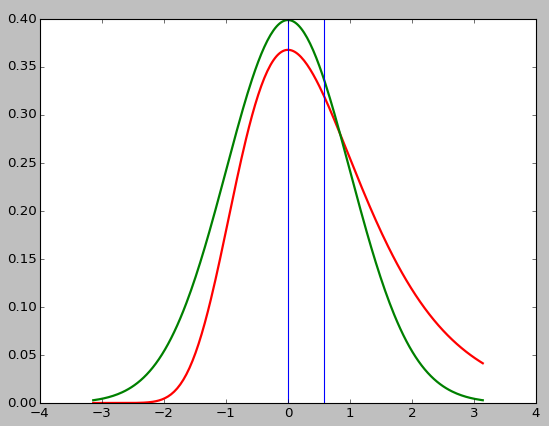
\includegraphics[width=0.5\textwidth]{images/gumbel_4.png}};

      %%   %% \draw[help lines,xstep=1,ystep=1] (0,0) grid (6,5);
      %%   %% \foreach \x in {0,1,...,5} { \node [anchor=north] at (\x,0) {\x,0};}
      %%   %% \foreach \y in {0,1,...,4} { \node [anchor=east] at (0,\y) {0,\y};}

      %%   \begin{scope}[x={(image.south east)},y={(image.north west)}]
      %%     %% \draw[red,ultra thick,rounded corners] (0.62,0.65) rectangle (0.78,0.75);
      %%     %% \path[draw,black,ultra thick] (3.1,0) -- (3.1,0.2);
      %%   \end{scope}
      %% \end{tikzpicture}
      %% %% %% %% \begin{minipage}{0.45\textwidth}
      %% %% %% %%   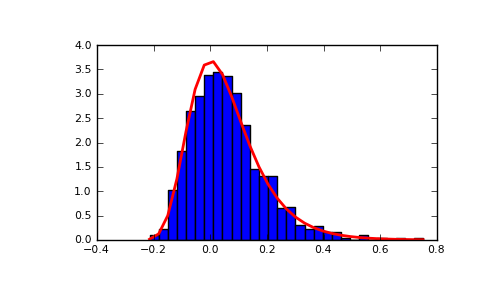
\includegraphics[height=5cm,width=6cm]{images/gumbel.png}
      %% %% %% %% \end{minipage}
      %% %% %% %% \hfill
      %% %% %% %% \begin{minipage}{0.45\textwidth}
      %% %%   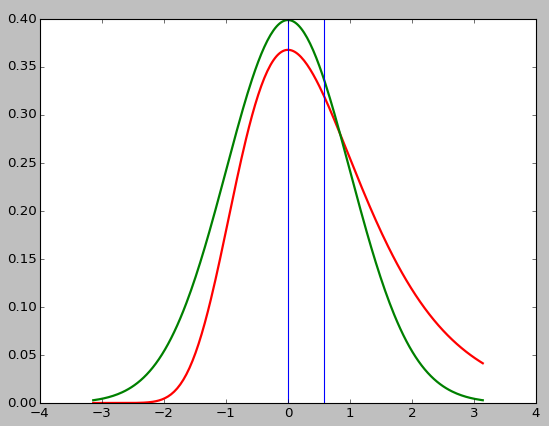
\includegraphics[scale=0.4]{images/gumbel_4.png}
      %% %% %% %% \end{minipage}
      \end{figure}   
    
\end{frame}

%%%%%%%%%%%%%%%%%%%%%%%%%%%%%%%%%%%%%%%%%%%%%%%%%%
\begin{frame}{Motivation}
  %% motivation stems from a trick made possible by the gumbel distribution 
  \onslide<1->
  \begin{property}
      For $G(i) \sim Gumbel(0)$, and any $B \subseteq [n]$
      \begin{align*}
        \onslide<2->{
          & \max_{i \in B}{G(i)+\phi(i)} \sim Gumbel\left(\log \sum_{i \in B} \exp(\phi(i))\right) \tag{Max-Stability}\\
          %% max of perturbed gumbels is also gumbelly distributed
        }
        \onslide<3->{
          & \argmax_{i \in B}{G(i)+\phi(i)} \sim \frac{\exp(\phi(i))}{\sum_{i \in B} \exp(\phi(i))}
        }
        %% position of the optimas are distributed acc. to gibbs
        %% proof in \cite{hazan}
      \end{align*}
      Also the $\argmax \perp \max$.
  \end{property}

\end{frame}


\begin{frame}{Motivation}
  %% Suppose you have a discrete distribution specified by un-normalized log probabilities $\{\phi(i)\}_{i=1}^{k}$ over k configurations $\{x_1,\cdots,x_k\}$, i.e.,
  \onslide<1->
  \begin{usage}[The Gumbel Max-Trick]
      Drawing samples from following when given only $\phi(i)$,
      \begin{align}
        \Pr(x_i) = \frac{\exp\phi(i)}{\sum_j\exp\phi(j)} \tag{$i \in [k]$}
      \end{align}
      %% We can draw samples $x_i \sim \Pr$ from this distribution using the following procedure.
      \onslide<2->
      \begin{align*}
        & \text{Sample} \qquad G(i) \sim Gumbel(0) \text{ for } i=1..k\\
        & \text{then} \qquad \text{ Choose } x_j \text{ such that } j= \argmax_i \{G(i) +\phi(i)\}
      \end{align*}
      %% the argmax of the perturbed probabilities is distributed as eq.\ref{eq:gibbs} above
  \end{usage}
\end{frame}
%%%%%%%%%%%%%%%%%%%%%%%%%%%%%%%%%%%%%%%%%%%%%%%%%%
\begin{frame}{Benefits}
  %% Wait ... So What?
  %% All this is cute, but what is the benefit?
  \begin{itemize}[<+->]
  \item Partition Function estimation $\implies$ Computing (many) perturbed MAPs.
    %% We have reduced a to b. No need to compute the partition function, as long as you can compute the (perturbed) argmax!
    %% perturbation is un-normalized
  %% \item \emph{Exact} samples from the target distribution. % Note that the samples are exact. (No approximations!)
    %% examples when things are approximations, MCMC ``once the chain reaches stationary distribution''
  \end{itemize}
  
  \begin{itemize}[<+->]
  \item \textsc{Question:} What if $k$ is large?
  \item \textsc{Question:} What happens if we move from discrete to continuous space?
  \item \textsc{Question:} Is There A Gumbel Max Trick for Continuous Distributions?
  \item {\color{red} This paper --- Yes!}
    %% One that does not resort to making infinite exponential perturbations?
  \end{itemize}
\end{frame}

%%%%%%%%%%%%%%%%%%%%%%%%%%%%%%%%%%%%%%%%%%%%%%%%%%
\begin{frame}{The Gumbel Process}
    \footnotesize{
  \begin{definition}
    $\{G_\mu(B) \mid B \subseteq \Omega\}$ is a Gumbel Process if,
    \begin{align*} 
      & G_\mu(B) \sim Gumbel(\log \mu(B)) \tag{samples are regional maxes}\\
      & G_\mu(B) \perp G_\mu(B^c) \tag{regional maxes are independent}\\
      & G_\mu(A \cup B) = \max(G_\mu(A),G_\mu(B)) \tag{maxes are consistent}
    \end{align*}
  \end{definition}
  \begin{property}
    For a Gumbel Process, $\{ \max \{G_k \mid X_k \in B\} \mid B \subseteq \Omega\}$,
    \begin{align*}
      \max \{G_k \mid X_k \in B\} \sim Gumbel(log \mu(B)) \\
      \argmax \{G_k \mid X_k \in B\} \sim \frac{\exp(\phi(x))1_{x \in B}}{\mu(B)}
    \end{align*}
    
  \end{property}
  }
\end{frame}

%%%%%%%%%%%%%%%%%%%%%%%%%%%%%%%%%%%%%%%%%%%%%%%%%%
\begin{frame}{Top-Down Construction of Gumbel Process}
    \visible<1->{
  \begin{figure} 
    \centering
    \begin{tikzpicture}[scale=0.7]
      %% \draw[step=0.5,gray] (-5,-3) grid (5,3);
      \path[draw,black,ultra thick] (-5,0)--(6,0);
      \onslide<1>
      \node[below] at (3,0) {$\Omega$};

      \onslide<2->
      \path[draw,red,thick] (2.5,0) -- (2.5,4.0) circle (1.5pt);
      \node[below] (x1) at (2.5,0) {$X_1$};
      \node[above] (g1) at (2.5,4.0) {$G_1$};

      \onslide<2-3>{
       \node[below] at (0.5,0) {\color{gray}{\small{$B$}}}; 
      }
      \onslide<2-3>{
        \node[below] at (4.0,0) {\color{gray}{\small{$B^c$}}};
      }

      \onslide<3->
      \path[draw,red,thick] (-2.0,0) -- (-2.0,3.0) circle (1.5pt);
      \node[below] (x2) at (-2.0,0) {$X_2$};
      \node[above] (g2) at (-2.0,3.0) {$G_2$};
      \only<3>\path[draw,blue,dotted,ultra thick,->] (2.5,4.0) -- (-2.0,3.0);

      \onslide<4->
      \path[draw,red,thick] (5.0,0) -- (5.0,-1.5) circle (1.5pt);
      \node[above] at (5.0,0) {$X_3$};
      \node[below] at (5.0,-1.5) {$G_3$};
      \only<4>\path[draw,blue,dotted,ultra thick,->] (2.5,4.0) -- (5.0,-1.5);

      \onslide<5->
      \path[draw,red,thick] (-1.0,0) -- (-1.0,1.5) circle (1.5pt);
      \node[below] at (-1.0,0) {$X_4$};
      \node[above] at (-1.0,1.5) {$G_4$};
      \only<5>\path[draw,blue,dotted,ultra thick,->] (-2.0,3.0) -- (-1.0,1.5);

      \onslide<6->
      \path[draw,red,thick] (-3.5,0) -- (-3.5,0.5) circle (1.5pt);
      \node[below] at (-3.5,0) {$X_5$};
      \node[above] at (-3.5,0.5) {$G_5$};
      \only<6>\path[draw,blue,dotted,ultra thick,->] (-2.0,3.0) -- (-3.5,0.5);
    \end{tikzpicture}
  \end{figure}
    }
  \begin{center}
    \visible<2>{
      $X_1 \sim \exp(\phi(x))/\mu(\Omega)$ \\% (global maximum)
      $G_1 \sim Gumbel(\log\mu(\Omega))$ \\
      %% and partition space accordingly
      
      %% \begin{align*}
      %%   & X_1 \sim \exp(\phi(x))/\mu(\Omega) \tag{assume $\log \mu(\Omega)$ is computable}\\
      %%   & G_1 \sim Gumbel(\log\mu(\Omega))
      %% \end{align*}
    }
    \visible<3>{
      $X_2 \sim \exp(\phi(x))1_{x \in B}/\mu(B)$ \\
      $G_2 \sim TruncGumbel(\log\mu(B),G_1)$ \\
      %% sample $X_2$ from partition $B$, and also sample the regional max $G_2$.
    }
    \visible<4>{
      %% Do same for other partition $B^c$,\\
      %% first sampling the argmax $X_i$ \\
      %% and then sampling its value $G_i$.
    }
    \visible<5->{
      %% Sample recursively.\\
      %% You now have a sequence of $(G_i,X_i)$ \\
      %% samples from the Gumbel Process.
    }
  \end{center}
  %% Assume log Z is computable for now.
\end{frame}

%%%%%%%%%%%%%%%%%%%%%%%%%%%%%%%%%%%%%%%%%%%%%%%%%%
\begin{frame}<1>[label=progress]{Progress So Far}
  \begin{itemize}[<+->]
  \item \textsc{Goal}: Drawing samples from target distribution $\Pr$.
  \item Reduction: $\argmax$ of sequence of (perturbed) Gumbel samples.
    %% We reduced it to computing argmax of a sequence of samples from a exotic distribution. % (because argmax follows the target dist)
  \end{itemize}
  \begin{overprint}

    \onslide<3>
    \textbf{Problems}
    \begin{itemize}
    \item {\color{red}Problem 1:} Computing $Z_{\Pr}$        % Drawing samples from the distribution requires knowing Z of my target distribution.
      %% \item {\color{red}Problem 2:} Drawing infinite samples to compute argmax on. % We do not want to draw infinite samples to compute argmax on.
    \end{itemize}

    \onslide<4>
    \textbf{Problems}
    \begin{itemize} 
    \item {\color{blue} Solution} Decompose! % I can draw samples from easier distribution, because I know its log Z. and then add the hard part to the samples before taking argmax.
    \item {\color{red} Problem 2:} Drawing infinite samples to compute argmax on. % We do not want to draw infinite samples to compute argmax on.
    \end{itemize}

    \onslide<5>
    \textbf{Problems}
    \begin{itemize} 
    \item {\color{blue} Solution} Decompose! % I can draw samples from easier distribution, because I know its log Z. and then add the hard part to the samples before taking argmax.
    \item {\color{blue} Solution} A* search.
    \end{itemize}
  \end{overprint}
\end{frame}

%%%%%%%%%%%%%%%%%%%%%%%%%%%%%%%%%%%%%%%%%%%%%%%%%%
\againframe<2-3>{progress}

%%%%%%%%%%%%%%%%%%%%%%%%%%%%%%%%%%%%%%%%%%%%%%%%%%
\begin{frame}{Solution - Perturbing Gumbel Processes} % Main Idea
  \begin{align*}
    \visible<1->{
      & \mu(B) = \int_{x\in B} \exp(\phi(x)) \tag{hard}\\
    }
    \visible<2->{
      & \nu(B)=\int_{x\in B} \exp(i(x)) \tag{easy}\\
    }
    \visible<3->{
      & \text{Let $o(x) = \phi(x) - i(x)$ be bounded}
    }    
  \end{align*}
  \visible<4->{
    \begin{property}
      If $G_k \sim Gumbel(\log\nu)$, then, $\{\max\{G_k + o(X_k) \mid X_k \in B\} \mid B \subseteq \R^d\}$ is a Gumbel Process with measure $\mu$.
    \end{property}
  }  
  \visible<5->{
    \emph{We can transform a Gumbel process into another by adding the difference of their log densities.} \\
  }
  %% So if I can easily draw samples from the prior and I have a way to compute the bound on the log-likelihood, then I can use Gumbel.
\end{frame}

%%%%%%%%%%%%%%%%%%%%%%%%%%%%%%%%%%%%%%%%%%%%%%%%%%
\againframe<3-4>{progress}

%%%%%%%%%%%%%%%%%%%%%%%%%%%%%%%%%%%%%%%%%%%%%%%%%%
\begin{frame}{Quick Review of A*}
  %% graph exploration strategy
  %% Uncover node in search space based on the following criteria
  Choose based on,
  \begin{overprint}
    \onslide<1>
    \begin{align*}
      \min_{n \in Q} f(n) = \min_{n \in Q} g(n) + h(n)
    \end{align*}
    \begin{itemize}
    \item g(n) distance from the start node to node n.
    \item h(n) \emph{estimate} of distance from node n to the goal node.
    %% optimistic for less cost
    \end{itemize}
    \onslide<2>
    \begin{align*}
      \max_{n \in Q} F(n) = \max_{n \in Q} G(n) + H(n)
    \end{align*}
    \begin{itemize}
    \item G(n) utility accumulated since the start node to node n.
    \item H(n) estimate of utility from node n to the goal node.
    %% optimistic for more reward 
    \end{itemize}
  \end{overprint}
\end{frame}

\begin{frame}{Main Idea}
  \begin{figure} 
    \centering
    \begin{tikzpicture}[scale=0.8]
      %% \draw[step=0.5,gray] (-5,-5) grid (5,5);

      \only<1>{
        \draw[ultra thick,gray] plot[smooth] coordinates {(-6,0) (5,0)};
      }
      
      \onslide<2->
      \draw[ultra thick,gray] plot[smooth] coordinates {(-6,0)(-5,0)(-3,3) (0,-1) (3,3) (5,0)};
      \node (ox) at (-4,-1) {o(x)};

      %% \begin{axis}[height=10cm,width=10cm]
      %%   \addplot[ultra thick,gray,smooth] coordinates {
      %%     (-6,0)(-5,0)(-3,3) (0,-1) (3,3) (5,0)}
      %%   node [pos=0.9,below left] {o(x)};
      %% \end{axis}
      
      \only<2>{
        \path[draw,dotted,blue,very thick] (-5,5.5) edge node[above] {upper bound} (5,5.5);
      }
      %% \addplot+[ycomb,black,thick] {1};
      %% \node[above] (g1) at (0,4) {};

      \onslide<2->{
        \path[draw,red,thick] (0,-1) -- (0,4) circle (1.5pt);
        \node[above] at (0,4.25) {$g_1+o(x_1)$};
      }
      
      \only<2,3>{
        \path[draw,green,dotted,very thick] (-5,4) edge node[below right] {\only<2>{lower bound}} (5,4);
      }
      
      \onslide<3->{
        \path[draw,red,thick] (-3,3) -- (-3,2) circle (1.5pt);
        \node[below] at (-3,1.5) {$g_2+o(x_2)$};
        \path[draw,red,thick] (3,3) -- (3,4.5) circle (1.5pt);
        \node[below] at (3,5.25) {$g_3+o(x_3)$};
      }

      \only<3,4>{
        \path[draw,dotted,blue,very thick] (-5,3.5) -- (0,3.5);
      }
      
      \only<3>{
        \path[draw,dotted,blue,very thick] (0,4.75) -- (5,4.75);
      }
      \only<4->{
        \path[draw,green,dotted,very thick] (-5,4.5) -- (5,4.5);
      }
      \only<4->{
        \path[draw,blue,dotted,very thick] (0,3.75) -- (3,3.75);
        \path[draw,blue,dotted,very thick] (3,3.25) -- (5,3.25);
        \path[draw,red,thick] (1.5,0.8) -- (1.5,0) circle (1.5pt);
        \path[draw,red,thick] (4,2) -- (4,0.5) circle (1.5pt);
      }
    \end{tikzpicture}
  \end{figure}  
\end{frame}

\begin{frame}{Experimental Results}
\end{frame}
